\chapter[Measurements]{Measurements}


The measurements can, to a certain extent, be broken into three main components: those pertaining to the solar wind, those from the magnetosphere in general, and those specific to the plasmasphere. An example of all the combined data sources is shown in Figure \ref{fig:alldata-GOES6-1983-1991}, providing solar wind variables $B_z$, $V_{SW}$; solar variable $F_{10.7}$, plasmatrough variable \req, and magnetosphere/plasmasphere variable \dst.

\vnote Include similar plot, but for single event

\begin{figure}
	\centering
	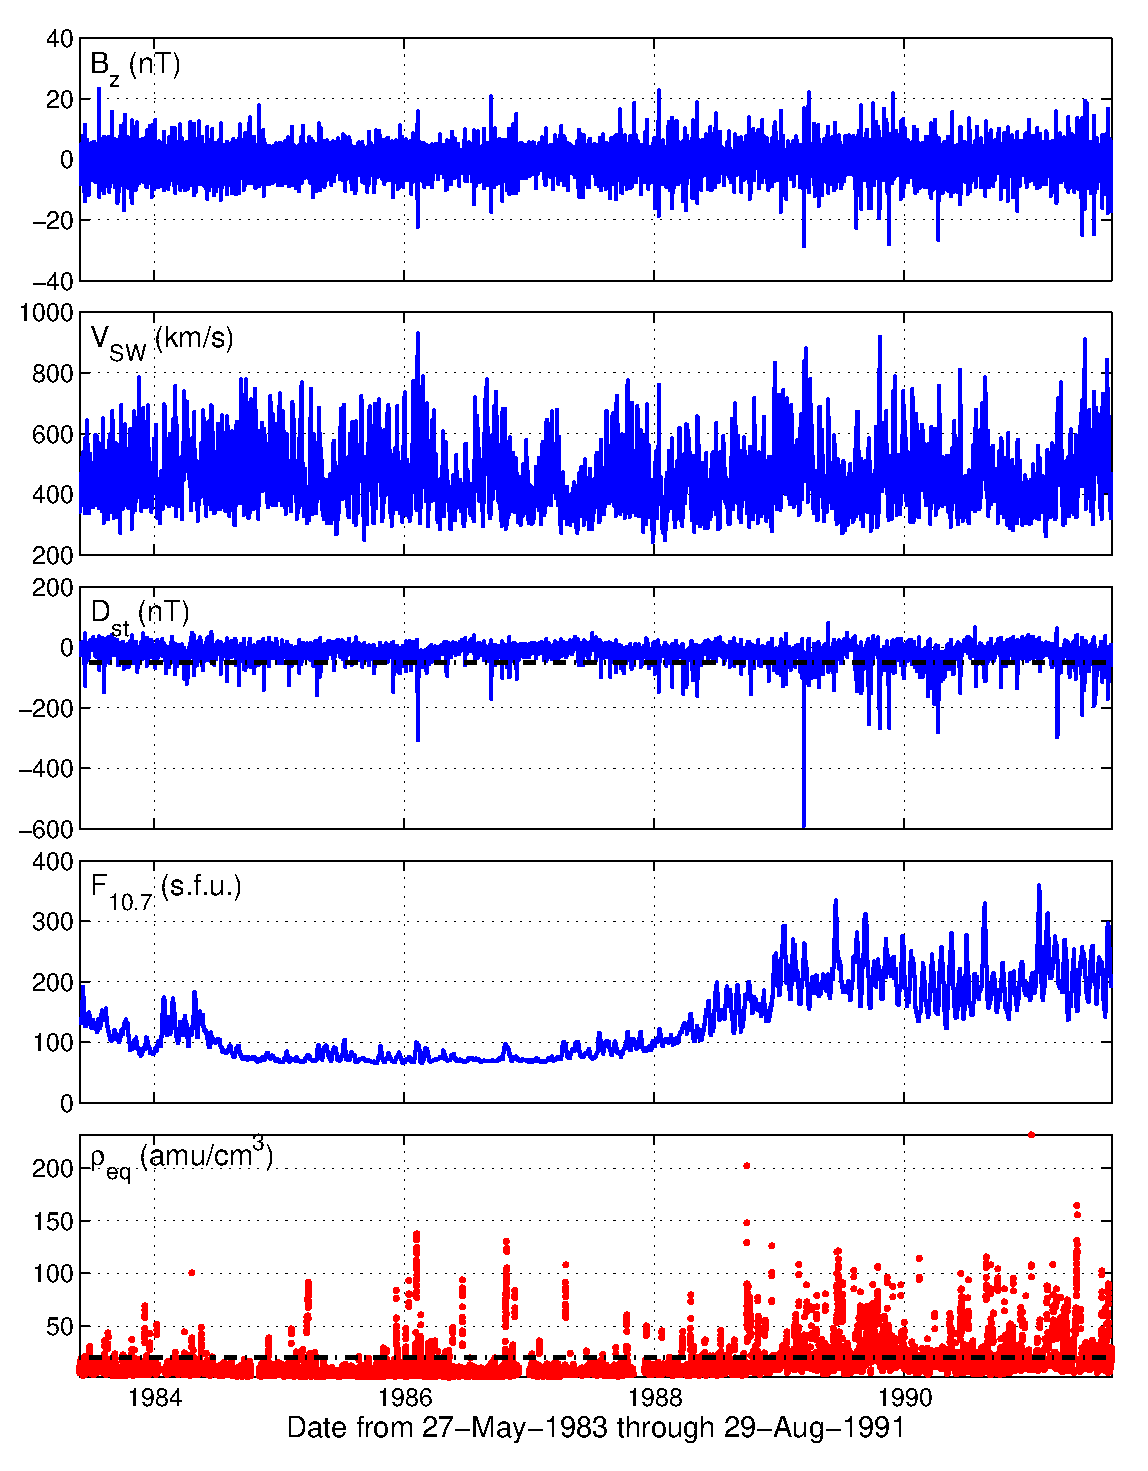
\includegraphics[width=0.7\linewidth]{Figures/alldata-GOES6-1983-1991}
	\caption{Selected data from GOES 6}
	\label{fig:alldata-GOES6-1983-1991}
\end{figure}

\section{Solar Wind}
Solar wind is the largest driver of particle density in the magnetosphere \vinote{cite}, and as such is an important input for a plasmatrough model. Conditions such as magnetic field orientation and particle velocity are important considerations for whether the plasmasphere is expected to be compressed, saturated, or experiencing high variability. By adding these to a model that account for time delayed inputs, their effects can be accounted for and aid in categorizing the state of the plasmatrough.

\subsection{Source}
Solar wind data for this dissertation is provided by the OMNIWeb service \vinote{cite}, a combination of many satellites' data to create a uniform, high resolution, near-Earth set of solar wind measurements. The one-hour resolution dataset was used since the study is concerned with effects on timescales of longer than an hour, and to more easily compare to the other data sources used. 

However, since the OMNIWeb data has gaps for some of the variables, \cite{Kondrashov2014ReconstructionOfGaps} was used as they reliably reconstruct gaps to make a continuous, uniform data set. \vinote{Details of how}

\subsection{Coverage}
Low resolution OMNI data is available from 1963 to present, but only the years of 1983-1992 were considered as they overlapped with the other data sets of interest. The data covers, but is not limited to: magnetic field strength in all three dimensions; solar wind proton density and temperature; the $K_p$, $AE$, $F_{10.7}$, and $D_{st}$ indices; and varying levels of proton flux.

\subsection{Data preparation}
The only data cleaning required on the OMNI dataset was to convert fill values of 999.9 and 9999 to NaN, to be appropriate for use in data analysis. Of the variables included (see Coverage), this was necessary for all variables other than $K_p$ and the proton flux variables.

\section{Geomagnetic}
Geomagnetic data cover everything inside the magnetopause, but in this study will tend to refer specifically to information in the magnetosphere but not in the plasmasphere or ionosphere.

\subsection{Source}
The data come from \cite{Takahashi2010SolarCycleVariation}, which takes data from the Geostationary Operational Environmental Satellites (GOES) and uses a set of magnetic field models to relate Alfvén waves to equatorial mass density (\req). \vinote{Define Alfvén waves? Earlier}. 

\subsection{Coverage}
The GOES satellites used in this study cover the years from 1980 to the end of 1991, often with overlapping years between satellites. The satellites themselves held a geostationary orbit at around 6.62 $R_E$ and collected data on a roughly 3-second cadence \citep{GOESDataSource}, which was then transformed onto a 10-minute cadence. Their position means they're almost always measuring properties of the plasmatrough, the region devoid of dense plasma just outside the plasmasphere.

\subsection{Data preparation}
The data were prepared by replacing fill values of 9999 with NaN and then narrowing results to only one satellite at a time to ideally remove any effects of satellite position or calibration from the results. These data still had many temporal gaps, so they were scaled onto a uniform 10-minute grid leaving missing points as NaN, but allowing for easier data analysis and comparison to other data sets.

In order to align the GOES data with the OMNI 1-hour cadence, the median of all existing values within 30 minutes on either side of each hour was taken. For hours with no existing values, a NaN was inserted to keep the cadence uniform. Two other methods were attempted: using the mean of each hour, centered on the hour, and using the median of the data on or within an hour after each time point (e.g. 7:00-7:59 would be combined into the 7:00 point). Both were found to have minimal effect on results.

\section{Plasmasphere}
Plasmasphere data covers the inner regions of the magnetosphere, bounded by the plasmapause on the outer edge and the ionosphere on the inner edge. This puts it at a typical distance of $L=3-5R_E$. 

\subsection{Source}
Data for the plasmasphere also comes from the GOES and OMNI datasets previously discussed, but have been calculated as extensions of directly measured data either onboard the satellites or from ground stations. 

\subsection{Coverage}
Since the data come from the same sources, the coverage is also the same. 
\vnote True? Any caveats, like specific MLT that calculations apply to plasmasphere?

\subsection{Data preparation}
See previous section. \vinote{Talk about specifics of calculations for plasmasphere variables? }
